\documentclass[12pt]{article}

\usepackage[margin=1in]{geometry} 
\usepackage{amsmath,amsthm,amssymb,enumitem,bbm,xparse,url,graphicx}

\newcommand{\N}{\mathbb{N}}
\newcommand{\Z}{\mathbb{Z}}
\newcommand{\R}{\mathbb{R}}
\newcommand{\Rd}{\mathbb{R}^{d}}
\newcommand{\exr}{[-\infty, \infty]}
\newcommand{\Biggnorm}{\Big | \Big |}

\NewDocumentCommand\closure{sm}
  {\IfBooleanTF{#1}{\overline{#2}}{\bar{#2}}}

\newenvironment{ex}[2][Exercise]{\begin{trivlist}
\item[\hskip \labelsep {\bfseries #1}\hskip \labelsep {\bfseries #2.}]}{\end{trivlist}}

\newenvironment{sol}[1][Solution]{\begin{trivlist}
\item[\hskip \labelsep {\bfseries #1:}]}{\end{trivlist}}

\newenvironment{theorem}[2][Theorem]{\begin{trivlist}
\item[\hskip \labelsep {\bfseries #1}\hskip \labelsep {\bfseries #2.}]}{\end{trivlist}}
    
\newenvironment{lemma}[2][Lemma]{\begin{trivlist}
\item[\hskip \labelsep {\bfseries #1}\hskip \labelsep {\bfseries #2.}]}{\end{trivlist}}
    
\newenvironment{definition}[2][Definition]{\begin{trivlist}
\item[\hskip \labelsep {\bfseries #1}\hskip \labelsep {\bfseries #2.}]}{\end{trivlist}}
    
\newenvironment{example}[1][Example]{\begin{trivlist}
\item[\hskip \labelsep {\bfseries #1:}]}{\end{trivlist}}
\begin{document}
\noindent David Owen Horace Cutler \hfill {\Large Math 237: Midterm} \hfill \today



\begin{ex}{1}
    Let $(X, \rho)$ be a compact metric space and $f: X \rightarrow X$ be a function such that
    $$\rho(f(x), f(y)) < \rho(x,y) \quad \forall x \neq y.$$
    Define $g : X \rightarrow \mathbb{R}$ by $g(x) = \rho(x, f(x))$. 
    \begin{enumerate}[label=(\alph*)]
        \item Prove that $g$ is Lipschitz function, and that $g$ has a minimum value that is achieved at a point $x \in X$. Conclude that there exists an $x \in X$ such that $g(x) = 0$.
        \begin{proof}
            We first want to show that $g$ is  Lipschitz, i.e. $\exists K \geq 0$ such that $\forall x, y \in X$ we have
            $$|g(x) - g(y)| \leq K\rho(x,y).$$
            As $X$ is a metric space then, the reverse triangle inequality holds. In particular we note that 
            $$|\rho(x, f(x)) - \rho(x, f(y))| = |\rho(f(x), x) - \rho(f(y), x)| \leq \rho(f(x), f(y)),$$
            and
            $$|\rho(x, f(y)) - \rho(y, f(y))| \leq \rho(x, y).$$
            We get then that 
            \begin{align*}
                |g(x) - g(y)| &= |\rho(x, f(x)) - \rho(x, f(y))| \\ 
                &= |\rho(x, f(x)) - \rho(x, f(y)) + \rho(x, f(y)) - \rho(y, f(y))| && \text{(Introducing a term)} \\
                &\leq |\rho(x, f(x)) - \rho(x, f(y))| + |\rho(x, f(y)) - \rho(y, f(y))| && \text{(Triangle inequality)} \\
                &\leq \rho(f(x), f(y)) + \rho(x, y) && \text{(Reverse triangle inequality)} \\
                &< 2\rho(x,y) && \text{(Definition of }f)
            \end{align*}
            It follows that $g$ is Lipschitz with Lipschitz constant $2$. Note here we are implicitly using $x \neq y$ to conclude the last part, but this isn't a problem as when $x = y$ as regardless we have
            $$0 = |g(x) - g(y)| \leq 2\rho(x, y) = 0$$
            As $g$ is Lipschitz then, it is continuous on $X$. It folows the \textbf{Extreme Value Theorem}\footnote{As stated on the Wikipedia article in the references.} is applicable, as $X$ is a compact metric space. In particular, this means $g$ achieves a minimum, i.e. at some point $x_0$.  \\ \\
            For the last part then, We claim then that $g(x_0) = 0$. To show this, we assume for the sake of contradiction that $g(x_0) \neq 0$. \\ \\
            By definition then, it must be $g(x_0) > 0$ then, i.e. 
            $$g(x_0) = \rho(x_0, f(x_0)) > 0.$$
            By the properties of the metric then, it must be $x_0 \neq f(x_0)$. We get then 
            $$g(f(x_0)) = \rho(f(x_0), f(f(x_0))) < \rho(x_0, f(x_0)) = g(x_0),$$
            which of course a contradiction as $g(x_0)$ should be the minimum value attained by $g$. Thus we must have $g(x_0) = 0$, which finishes off the proof.
        \end{proof}
        \item Show that $f$ has a unique fixed point $x_0$. 
        \begin{proof}
            By the previous part, there exists some $x_0$ such that $g(x_0) = 0$. Note then 
            \begin{align*}
                g(x_0) = 0 \\
                \longrightarrow \rho(x_0, f(x_0)) = 0 \\
                \longrightarrow x_0 = f(x_0)
            \end{align*}
            where the last deduction comes from properties of the metric. Thus $f$ has a fixed point $x_0$. \\ \\
            We want to argue uniqueness then, so assume for the sake of contradiciton there is an $x_1 \in X$ such that $f(x_1) = x_1$, where $x_1 \neq x_0$. \\ \\
            Here we get 
            $$\rho(x_0, x_1) = \rho(f(x_0), f(x_1)) < \rho(x_0, x_1)$$
            which is of course a contradiction. It follows $f$ has unique fixed point $x_0$.
        \end{proof}
        \item Show that the assumption that $X$ is compact cannot be ommited. 
        \begin{proof}
            Simply consider $f: (0,1) \rightarrow (0,1)$ defined by 
            $$x \mapsto \frac{x}{2},$$
            where $(0,1)$ is equipped with the standard metric. Then we get for $x, y \in (0,1)$ where $x \neq y$ that
            $$|f(x) - f(y)| = \Big|\frac{x}{2} - \frac{y}{2} \Big| = \frac{1}{2}|x - y| < |x - y|,$$
            so $f$ fulfills the given property. However, $f$ trivially has no fixed point, as the only candidate is $0$, which is not in the interval.
        \end{proof}
    \end{enumerate}
\end{ex}

\begin{ex}{2}
    Let $X$ and $Y$ be Banach spaces. Show that $T \in L(X,Y)$ is surjective if and only if $\text{range}(T)$ is not meager in $Y$. 
    \begin{proof}
        We will verify that $T \in L(X,Y)$ is surjective if and only if $\text{range}(T)$ is not meager in $Y$.
        \begin{enumerate}[label=(\roman*)]
            \item \textit{(Surjectivity has range is not meager)} Assume for the sake of contradiction that $\text{range}(T)$ is meager.  \\ \\
            As $T$ is surjective, clearly 
            $$\text{range}(T) = Y,$$
            where $Y$ is is Banach. By the \textbf{Baire Category Theorem} then, it should be $Y$ is a nonmeager subset of itself. \\ \\
            But then clearly this is a contradiction, as we assume $\text{range}(T) = Y$ is meager. It follows $\text{range}(T)$ must be not meager.
            \item \textit{(Range is not meager has surjectivity)} 
            Let $B_n^X(0)$ denote the ball of radius $n$ about the origin in $X$.  \\ \\
            As the norm is finite then, of course we have 
            $$X = \bigcup_{n = 1}^\infty B_n^X(0),$$
            and as the image of a union is the union of images, we get 
            $$\text{range}{(T)} = T(X) = T \Big (\bigcup_{n = 1}^\infty B_n^X(0) \Big) = \bigcup_{n = 1}^\infty T(B_n^X(0)).$$
            Linearity of $T$ immediately has that $T(B_n^X(0)) = nT(B_1^X(0))$, where $nT$ is the bounded, linear operator defined by $(nT)(n) = nT(n)$. \\ \\
            Thus we can additionally refine 
            $$\text{range}{(T)} = \bigcup_{n = 1}^\infty T(B_n^X(0)) = \bigcup_{n = 1}^\infty nT(B_1^X(0)),$$
            and so as $\text{range}(T)$ is nonmeager, it must be that some $nT(B_1^X(0))$ is \textit{not} nowhere dense, i.e. for some $n \in N$ we have that $\overline{nT(B_1^X(0))}$ has nonempty interior. \\ \\
            As we noted $nT$ is a bounded linear transformation then, we appeal to \textbf{Theorem 2.26} in Heil's \textit{A Basis Theory Primer}, which has that there exists an $r > 0$ such that 
            $$B_r^Y(0) \subseteq nT(B_1^X{0}).$$
            Let $y \in Y$ then. We see that $\frac{ry}{2||y||} \in B_r^Y(0)$. Using then that $B_r^Y(0) \subseteq nT(B_1^X{0})$ then, it is that 
            $$\frac{ry}{2||y||} = nT(x),$$
            for some $x$ in the unit ball in $X$. We organize then to get 
            $$y = \frac{2||y||}{r}nT(x) = \frac{2||y||n}{r}T(x) = T \Big (\frac{2||y||n}{r}x \Big),$$
            and so $y \in \text{range}(T)$. Thus $T$ is surjective.
        \end{enumerate}
        With both directions verified then, we get the desired result.
    \end{proof}
\end{ex}

\begin{ex}{3}
    Let $C_b(\mathbb{R})$ be the space of bounded, continuous functions, and let $C_b^1(\mathbb{R})$ be the space of functions such that $f, f' \in C_b(\mathbb{R})$. Equip both of these spaces with the uniform norm. 
    \begin{enumerate}[label=(\alph*)]
        \item Prove that $C_b(\mathbb{R})$ is complete but $C_b^1(\mathbb{R})$ is not. 
        \begin{proof}
            We first move to prove that $C_b(\mathbb{R})$ is complete. To accomplish this, we reproduce the proof of \textbf{Theorem 1.3.3} in Heil's \textit{Introduction to Real Analysis}.
            \begin{enumerate}[label=(\roman*)]
            \item $(C_b(\mathbb{R})$\textit{ is complete})
            Let $\{f_n\}_{n = 1}^\infty \subseteq C_b(\mathbb{R})$ be Cauchy in the uniform norm. Fixing some specific point $x$ in $\mathbb{R}$, we note of course that for any given $n$ and $m$ we have
            $$|f_n(x) - f_m(x)| \leq ||f_m - f_n||_u$$
            and so $\{f_n(x)\}_{n = 1}^\infty$ is a Cauchy sequence in our codomain, i.e. $\mathbb{R}$ or $\mathbb{C}$. However, both of these spaces are complete, so the sequence $\{f_n(x)\}_{n = 1}^\infty$ must converge. \\ \\
            Define the the function $f$ by stipulating
            $$f(x) = \underset{n \rightarrow \infty}{\lim} f_n(x),$$
            we claim that $f_n \xrightarrow{u} f$, i.e. $f_n$ converges to $f$ \textit{uniformly}. \\ \\
            For this sake, let $\epsilon > 0$. Using the Cauchyness of $\{f_n\}_{n = 1}^\infty$ in the uniform norm, we know there exists an $N$ such that 
            $$||f_n - f_m||_u < \epsilon \text{ for } n, m \geq N,$$
            and thus if $m \geq N$ we have for every $x \in \mathbb{R}$ that 
            $$|f(x) - f_m(x)| = \underset{n \rightarrow \infty}{\lim} \; |f_n(x) - f_m(x)| \leq \underset{m \rightarrow \infty}{\lim \sup} \; ||f_m - f_n||_u \leq \epsilon.$$
            We can take the supremum over all $x \in \mathbb{R}$ to get $||f - f_m||_u \leq \epsilon$ for $m \geq N$, and so it follows $f_n \rightarrow f$ uniformly. \\ \\
            In addition to this, the \textbf{Uniform Limit Theorem} tells us that $f$ is continuous on $\mathbb{R}$, as all the $f_n$ are. Moreover, $f$ is bounded as all the $f_n$ are, given that 
            $$||f||_u \leq ||f - f_n + f_n||_u \leq ||f - f_n||_u + ||f_n||_u,$$
            and so taking $||f - f_n||_u$ small shows that $||f||_u$ bounded. It follows $f \in C_b(\mathbb{R})$, where $f_n \xrightarrow{u} f$. Thus $C_b(\mathbb{R})$ is complete.
            \item $(C_b^1(\mathbb{R})$\textit{ is not complete}) We define a sequence of functions $\{f_n\}_{n = 1}^\infty$ in the following way:
            $$f_n(x) = \sum_{k = 0}^n 2^{-k}\cos(13^k \pi x)$$
            We can establish $\{f_n\}_{n = 1}^\infty \subseteq{C_b^1(\mathbb{R})}$ by showing $f_n$ and $f'_n$ are bounded for each $n$. Let $n \in N$ then. For $f$ then we note 
            \begin{align*}
            |f_n(x)| = \Big | \sum_{k = 0}^n 2^{-k}\cos(13^k \pi x) \Big | \leq \sum_{k = 0}^n |2^{-k}\cos(13^k \pi x)| \\
            \leq \sum_{k = 0}^n 2^{-k} < \sum_{k = 0}^\infty 2^{-k} = 2,
            \end{align*}
            and for $f'$ we have 
            \begin{align*}
                |f'_n(x)| = \Big | \sum_{k = 0}^n -\pi \Big (\frac{13}{2} \Big)^k \sin(13^k \pi x) \Big | \leq \sum_{k = 0}^n \Big | \pi \Big (\frac{13}{2} \Big)^k \sin(13^k \pi x) \Big | \\
                \leq \sum_{k = 0}^n \pi \Big (\frac{13}{2} \Big)^k < \infty,
            \end{align*}
            so both $f_n$ and $f'_n$ are bounded. Additionally, it is evident both $f_n$ and $f'_n$ are continuous. It follows $\{f_n\}_{n = 1}^\infty \subseteq C_b^1(\mathbb{R})$. \\ \\
            Moreover, we can verify this sequence is uniformly Cauchy, taking $N$ where $n, m \geq N$ and with $n > m$ without loss of generality. Then for any $x \in \mathbb{R}$ we get
            \begin{align*}
                |f_n(x) - f_m(x)| = \Big | \sum_{k = 0}^n 2^{-k}\cos(13^k \pi x) - \sum_{k = 0}^m 2^{-k}\cos(13^k \pi x) \Big | \\
                \leq \Big | \sum_{k = m + 1}^n 2^{-k}\cos(13^k \pi x) \Big | \leq \sum_{k = m + 1}^n 2^{-k} \leq \sum_{k = N}^n 2^{-k},
            \end{align*}
            where taking $N \rightarrow 0$ thus shows Cauchyness, and the last sum gets arbitrarily small. As this bound is not dependent on $x$, taking the supremum over all $x$ has the sequence is uniformly Cauchy. \\ \\
            However, this is an issue as this sequence of functions is precisely the definition of a \textbf{Weierstrass Function}\footnote{See Brent Nelson's online notes titled \text{``The Weierstrass Function"} for proof of uniform convergence to a nonwhere differentiable function. Listed in references.}, as $\frac{1}{2}(13) > \frac{3\pi}{2}$. Thus its limit is not in $C_1^b(\mathbb{R})$, as it is nowhere differentiable. \\ \\
            Appealing to uniqueness of the uniform limit then, it follows $C^1_b(\mathbb{R})$ is not complete as $\{f_n\}_{n = 1}^\infty \subseteq C^1_b(\mathbb{R})$ is a Cauchy sequence with no limit in $C_b^1(\mathbb{R})$.
            \end{enumerate}
        \end{proof}
        \item Show that the differentiation operator $D: C_b^1(\mathbb{R}) \rightarrow C_b(\mathbb{R})$ given by $Df = f'$ is unbounded, but has a closed graph.
        \begin{proof}
            \begin{enumerate}[label=(\roman*)]
            We need to show $D$ is unbounded but that it has a closed graph.
            \item \textit{(D is unbounded)} To show $D$ is unbounded, it is sufficient to show there is a bounded sequence $\{f_k\}_{k = 1}^\infty$ that has $\{Df_k\}_{k = 1}^\infty$ unbounded. \\ \\ 
            For this, consider the sequence such that $f_k = \sin(kx)$. Of course for each $k$ we have 
            $$||f_k||_u = 1,$$
            but we note $Df_k = k\cos(kx)$. But then $Df_k(0) = k\cos(k \cdot 0) = k$. Of course
            $$k = |Df_k(0)| \leq ||Df_k||_u,$$
            which clearly has that $\{Df_k\}_{k = 1}^\infty$ is unbounded, taking $k \rightarrow \infty$.
            \item \textit{(D has a closed graph)} Let $f_k \xrightarrow{u} f \in C_b^1(\mathbb{R})$ and let $Df_k \xrightarrow{u} g \in C_b(\mathbb{R})$, i.e. $f'_k \xrightarrow{u} g \in C_b(\mathbb{R})$. To show $D$ has a closed graph, we need to show $Df = f' = g$. \\ \\
            For this, consider an arbitrary compact interval $[a,b]$. As we have $f'_k \xrightarrow{u} g$ uniformly on $\mathbb{R}$, we have uniform convergence on $[a,b]$, and consequently $L^1$ convergence. \\ \\ In particular we note, considering the indefinite integral on $[a,b]$ that
            $$\underset{k \rightarrow \infty}{\lim} \int_a^x f'_k = \int_a^x g$$
            As $f$ is $C^1$ then, the \textbf{Fundamental Theorem of Calculus} is applicable, i.e. 
            $$\underset{k \rightarrow \infty}{\lim} f_k(x) - f_k(a) = \underset{k \rightarrow \infty}{\lim} \int_a^x f'_k = \int_a^x g,$$
            where $f_k \xrightarrow{u} f$ additionally has pointwise convergence, so get we finally 
            $$f(x) - f(a) = \int_a^x g.$$
            We can apply then the second statement of the \textbf{FTC}, given the continuity of $g$, to get
            $$f'(x) =  D(f(x) - f(a)) = D \Big ( \int_a^x g \Big ) = g(x),$$
            and as this holds over all compact intervals, we can extrapolate to get $f' = g$ in general. Thus $Df = f' = g$, and so we have a closed graph.
            \end{enumerate}
        \end{proof}
    \end{enumerate}
\end{ex}

\begin{ex}{4}
    Let $H = L^2([0,1], \mathbb{R})$ be the space of all real-valued Lebesgue measurable and square-integrable functions on $[0,1]$. Let $K$ be a nonempty closed convex subset of $H$, and $P = P_K$ be the orthogonal projection of $H$ onto $K$.
    \begin{enumerate}[label=(\alph*)]
        \item Let $x \in H$. Prove that the following two statements are equivalent.
        \begin{enumerate}[label=(\roman*)]
            \item There exists a unique $z \in K$ such that $||x - z|| = \underset{y \in K}{\min} \; ||x - y||$. 
            \item The vector $z$ in (i) is characterized by
                \begin{equation*}
                \begin{cases}
                    z \in K \\
                    \langle x - z, y - z \rangle \leq 0 & \forall y \in K
                \end{cases}
                \end{equation*}
                \begin{proof}
                    We start with the forward direction, assuming (i) and hoping to show (ii). With this in mind, let $y \in K$. We define $y_t$ by stipulating
                    $$y_t = (1 - t)z + ty \text{ for } t \in (0,1)$$
                    we note $y_t \in K$ for $t \in (0,1)$, as $z, y \in K$ and $K$ is convex. Thus by assumption 
                    $$||x - z|| \leq ||x - y_t||.$$
                    We get the following derivation then, making extensive use of the properties of the inner product:
                    \begin{align*}
                        ||x - z||^2  \leq ||x - y_t||^2 
                        = ||x - (1 - t)z - ty||^2 \\
                        = ||x - z + tz - ty||^2 
                        = \langle x - z + tz - ty, x - z + tz - ty\rangle \\
                        = \langle x - z, x - z + tz - ty \rangle + \langle tz - ty, x - z + tz - ty \rangle \\
                        = \langle x - z, x - z \rangle + \langle x - z, tz - ty\rangle + \langle tz - ty, x - z \rangle + \langle tz - ty, tz - ty \rangle \\
                        = ||x - z||^2 + ||tz - ty||^2 + 2t\langle x - z, z - y \rangle
                    \end{align*}
                    We can rewrite this even more to get 
                    $$||x - z||^2 \leq ||x - z||^2 + t^2||z - y||^2 - 2t\langle x - z, y - z\rangle,$$
                    i.e. 
                    $$\langle x - z, y - z\rangle \leq \frac{t}{2}||z - y||^2.$$
                    Taking $t \rightarrow 0$ then gets that 
                    $$\langle x - z, y - z\rangle  \leq 0,$$
                    where then this holds for all $y \in K$ given our arbitrary choice of $y \in K$. \\ \\
                    Assume then (ii) (i.e. consider $z$ with the outlined properties), we want to show (i). Let $y \in K$; we get the following:
                    \begin{align*}
                        \langle x - z, y - z \rangle = \langle x - z, y - x + x - z \rangle \\
                        = \langle x - z, y - x \rangle + \langle x - z, x - z \rangle \\
                        = ||x - z||^2 + \langle x - z, y - z \rangle \\
                        = ||x - z||^2 - \langle x - z, x - y \rangle
                    \end{align*}
                    By our assumption then we have 
                    $$||x - z||^2 - \langle x - z, x - y \rangle \leq 0,$$
                    and so we can rearrange to get 
                    $$||x - z||^2 \leq \langle x - z, x - y \rangle.$$
                    Applying Cauchy-Schwarz thus gets
                    \begin{align*}
                        ||x - z||^2 \leq \langle x - z, x - y \rangle \leq |\langle x - z, x - y \rangle| \leq ||x - z||||x - y|| \\
                        \longrightarrow ||x - z|| \leq ||x - y||,
                    \end{align*}
                    and so as $y \in K$ was arbitrary we have $||x - z|| \leq \underset{y \in K}{\min} ||x - y||$, with $z \in K$ by assumption. \\ \\
                    We want to argue uniqueness of this $z$ then. For this, suppose we have some $z' \in K$ fulfilling the same inequality. \\ \\
                    Clearly then, we have
                    $$||x - z|| \leq ||x - z'|| \text{ and } ||x - z'|| \leq ||x - z||,$$
                    so $||x - z|| = ||x - z'||$. In addition we of course have 
                    $$\frac{x - z}{||x - z||} = \frac{x - z'}{||x - z'||} = 1,$$
                    so the strict convexity of the unit ball with respect to the $L^2$ norm (as proven in the first homework) has for $t \in (0,1)$ that 
                    $$\Biggnorm t\frac{x - z}{||x - z||} + (1 - t)\frac{x - z'}{||x - z'||} \Biggnorm < 1.$$
                    As $||x - z|| = ||x - z'||$ then, we can multiply by $||x - z||$ to get the following:
                    $$||t(x - z) + (1 - t)(x - z')|| < ||x - z||$$
                    But this presents an issue, as we note 
                    \begin{align*} 
                        t(x - z) + (1 - t)(x - z') \\
                        = x + tz' - tz - z' \\
                        = x - (tz + z' - tz') \\
                        = x - (tz + (1 - t)z')
                    \end{align*}
                    So we have 
                    $$||x - (tz + (1 - t)z')|| < ||x - z||,$$
                    but this is a problem as $z, z' \in K$, so $(tz + (1 - t)z') \in K$ for $t \in (0,1)$ by convexity. \\ \\
                    We therefore get a contradiction, as it should then of course be (as $z$ minimizes the distance) that we have 
                    $$||x - z|| \leq ||x - (tz + (1 - t)z')||.$$
                    It follows the point $z$ must be unique then, so we have (i). As we have shown both directions then, the two statements are equivalent.
                \end{proof}
        \end{enumerate}
        \item Let $A$ be a continuous bilinear mapping from $H \times H$ into $\mathbb{R}$ such that for some $\alpha > 0$ we have
         $$A(f, f) \geq \alpha||f||_2^2 \; \forall f \in H$$
        \begin{enumerate}[label=(\arabic*)]
            \item Fix $u \in H$ and prove that there exists a unique $Tu \in H$ such that $A(u,v) = \langle Tu, v \rangle$ for all $v \in H$. Prove that $T$ is a bounded linear mapping on $H$.
            \begin{proof}
                Fix some $u \in H$, as $A$ is continuous on $H \times H$ and bilinear, it follows $A(u, \cdot)$ is continuous on $H$ and linear. \\ \\
                More specifically, $A(u, \cdot)$ is a bounded linear functional. It follows by the \textbf{Riesz Representation Theorem} that for some unique $z \in H$, we have 
                $$A(u, v) = \langle v, z \rangle \; \forall v \in H.$$
                Define then $T$ by stipulating $Tu = z$; the \textbf{RRT} also thus has $T$ is well-defined and $Tu$ is unique and the given $z$ must be unique. \\ \\
                We thus have for the unique $Tu \in H$ that
                $$A(u,v) = \langle v, Tu \rangle = \langle Tu, v \rangle \quad \forall v \in H.$$
                We want then to show in addition that $T$ is linear and bounded. We start by showing $T$ is linear, i.e. for $a, b \in \mathbb{R}$ and $x, y \in H$ we have 
                $$T(ax + by) = aT(x) + bT(y).$$
                Using the linearity of $A$ in the first argument we get that
                \begin{align*}
                    A(ax + by, v) = aA(x, v) + bA(y, v) \quad \forall v \in H
                \end{align*}
                so it by construction we have 
                \begin{align*}
                    \langle T(ax + by), v \rangle = a\langle T(x), v \rangle + b\langle T(y), v \rangle \quad \forall v \in H\\
                    \longrightarrow \langle T(ax + by), v \rangle = \langle aT(x) + bT(y), v \rangle \quad \forall v \in H \\
                    \longrightarrow \langle T(ax + by) - aT(x) - bT(y), v \rangle = 0 \quad \forall v \in H,
                \end{align*}
                but the only vector orthogonal to all other vectors is the zero vector, i.e. $T(ax + by) - aT(x) - bT(y) = 0$, so 
                $$T(ax + by) = aT(x) + bT(y).$$
                The last thing to show then is that $T$ is bounded; for this, we can show it has finite operator norm. \\ \\
                By our earlier working with \textbf{RRT}, we know for each $u$ that $||A(u, \cdot)||_{B(H, \mathbb{R})} = ||Tu||_H$. Thus we get 
                \begin{align*}
                    ||T||_{H^*} = \underset{||u||_H = 1}{\sup} ||Tu||_H = \underset{||u||_H = 1}{\sup} ||A(u, \cdot)||_{B(H, \mathbb{R})},
                \end{align*}
                where each $||A(u, \cdot)||_{B(H, \mathbb{R})}$ is finite, given each is bounded/continuous on $H$. We want now to apply the \textbf{Uniform Boundedness Principle} (note $H$ and $\mathbb{R}$ are Banach spaces). \\ \\  Let some $v \in H$, then 
                $$\underset{||u||_H = 1}{\sup} |A(u, \cdot)(v)| = \underset{||u||_H = 1}{\sup} |A(u, v)| = ||A(\cdot, v)||_{B(H,\mathbb{R})}$$
                by definition. Of course, the latter quantity is finite as fixing $A$ is one variable leads to a continuous/bounded linear function on $H$, and so it has finite operator norm. \\ \\
                Applying the \textbf{UBP} thus has
                $$\underset{||u||_H = 1}{\sup} ||A(u, \cdot)||_{B(H, \mathbb{R})} < \infty,$$
                and so consequently $||T||_{H^*} < \infty$, which is sufficient to determine that $T$ is bounded as we always have 
                $$||Tu||_H \leq ||T||_{H^*}||u||_H$$
                for $u \in H$. 
            \end{proof}
            \item Let $\rho > 0$ and define a mapping $S_\rho$ on $K$ given by $S_\rho v = P(\rho f, pTv + v)$ for $v \in K$. Prove that $\rho > 0$ can be chosen such that there exists $0 < k < 1$ with the property that 
            $$||S_\rho v_1 - S_\rho v_1|| \leq k||v_1 - v_2|| \quad \forall v_1, v_2 \in K$$
            \begin{proof}
                We need first to prove that the projection onto $K$ is Lipschitz with constant 1. \\ \\
                For this, consider $x, y \in H$. We want to show that 
                $$||Px - Py|| \leq ||x - y||.$$
                Assume then $x \neq y$, as $x = y$ is trivial. By our earlier work in (a) then, we thus have 
                \begin{align*}
                    \langle x - Px, Py - Px \rangle \leq 0 \\
                    \langle y - Py, Px - Py \rangle \leq 0,
                \end{align*}
                as $Px, Py \in K$. Working through this then, we get the following derivation:
                \begin{align*}
                    \langle x - Px, Py - Px \rangle + \langle y - Py, Px - Py \rangle \leq 0 \\
                    \longrightarrow \langle y - Py, Px - Py \rangle - \langle x - Px, Px - Py \rangle \leq 0 \\
                    \longrightarrow \langle y - Py, Px - Py \rangle + \langle Px - x, Px - Py \rangle \leq 0 \\
                    \longrightarrow \langle y - Py - x + Px, Px - Py \rangle \leq 0 \\
                    \longrightarrow \langle y - x + (Px - Py), Px - Py\rangle \leq 0 \\
                    \longrightarrow -\langle x - y, Px - Py\rangle + ||Px - Py||^2 \leq 0 \\
                    \longrightarrow ||Px - Py||^2 \leq \langle x - y, Px - Py \rangle 
                \end{align*}
                Thus, applying Cauchy-Schwarz we get
                $$||Px - Py||^2 \leq \langle x - y, Px - Py \rangle \leq ||x - y||||Px - Py||,$$
                and so
                $$||Px - Py|| \leq ||x - y||.$$
                With this in mind then, we move to prove the desired result. We note for $v_1, v_2 \in K$ then that 
                \begin{align*}
                    ||S_\rho v_1 - S_\rho v_2||^2 \\
                    = ||P(\rho f - \rho Tv_1 + v1) - P(\rho f - \rho Tv_2 + v2)||^2 \\
                    \leq ||(\rho f - \rho Tv_1 + v_1) - (\rho f - \rho Tv_2 + v_2)||^2 && \text{(Lipschitz with 1)} \\
                    = ||(v_1 - v_2) - \rho T(v_1 - v_2)||^2 \\
                    = ||v_1 - v_2||^2 - 2\rho \langle T(v_1 - v_2), v_1 - v_2 \rangle + ||\rho T(v_1 - v_2)||^2 && \text{(Expanding inner product)} \\
                    \leq ||v_1 - v_2||^2 - 2\rho \langle T(v_1 - v_2), v_1 - v_2 \rangle + \rho^2 ||T||^2||v_1 - v_2||^2 \\
                    = ||v_1 - v_2||^2 - 2\rho A(v_1 - v_2, v_1, v_2) + \rho^2 ||T||^2||v_1 - v_2||^2 \\
                    \leq ||v_1 - v_2||^2 - 2\rho \alpha ||v_1 - v_2||^2 + \rho^2 ||T||^2||v_1 - v_2||^2 && \text{(Inequality on }A)\\
                    = (1 - 2\rho\alpha + \rho^2||T||^2)||v_1 - v_2||^2
                \end{align*}
                Thus to get what we desired, we just need $(1 - 2\rho\alpha + \rho^2||T||^2) < 1$. Note then 
                \begin{align*}
                    (1 - 2\rho\alpha + \rho^2||T||^2) < 1 \\
                    \leftrightarrow \rho^2 ||T||^2 < 2\rho \alpha \\
                    \leftrightarrow \rho < \frac{2\alpha}{||T||^2}
                \end{align*}
                Thus choosing $\rho < \frac{2\alpha}{||T||^2}$ gets us a $k = (1 - 2\rho\alpha + \rho^2||T||^2) < 1$ for which we have 
                $$||S_\rho v_1 - S_\rho v_2||^2 \leq k||v_1 - v_2|| \quad \forall v_1, v_2 \in K$$
                as desired.
            \end{proof}
            \item Conclude that for the value of $\rho$ given in (2), that $S_p$ is a contraction, and thus has a unique fixed point $u \in K$. 
            \begin{proof}
                As our given $k$ in the last part is such that $k < 1$, $S_\rho$ is by definition a contraction. As $K$ is a closed subset of $H$ then and $H$ is complete, $K$ is a complete metric space. \\ \\
                Moreover, $S_\rho$ is a function $K \rightarrow K$. \\ \\
                By the \textbf{Banach Fixed Point Theorem}\footnote{As stated on the Wikipedia article in the references.} then, $S_\rho$ admits a unique fixed point $u \in K$.
            \end{proof}
            \item By writing $\rho f - \rho Tu = \rho f - \rho Tu + u - u$ and using part (a), show that 
            $$\langle \rho f - \rho Tu, v - u \rangle \leq 0 \quad \forall v \in K.$$
            \begin{proof}
                Let $v \in K$. Considering $w = \rho f + \rho Tu + u$ (with $u$ as produced in the last part) we get 
                $$Pw = P(\rho f + \rho Tu + u) = S_\rho(u) = u.$$
                As $u \in K$, we get by (1) that 
                \begin{align*}
                    \langle w - u, v - u \rangle \leq 0 \\
                    \longrightarrow \langle \rho f + \rho Tu, v - u \rangle \leq 0
                \end{align*}
                and so 
                $$\langle \rho f + \rho Tu, v - u \rangle \leq 0 \quad \forall v \in K,$$
                as desired.
            \end{proof}
            \item Conclude that given any $f \in H$, there exists a unique $u \in K$ such that 
            $$A(u, v - u) \geq \langle f, v - u \rangle \quad \forall v \in K.$$
            \begin{proof}
                Let $f \in H$ and consider some $v \in K$. Using the previous part then, we get the following:
                \begin{align*}
                    \langle \rho f - \rho Tu, v - u \rangle \leq 0 \\ 
                    \longrightarrow \rho(f - Tu, v - u) \leq 0 \\
                    \longrightarrow \langle f - Tu, v - u \rangle \leq 0 \\
                    \longrightarrow \langle f, v - u \rangle - \langle Tu, v - u \rangle \leq 0 \\
                    \longrightarrow \langle f, v - u \rangle \leq \langle Tu, v - u \rangle
                \end{align*}
                But note of course 
                $$\langle Tu, v - u \rangle = A(u, v -u),$$
                so we get
                $$\langle f, v - u \rangle \leq A(u, v - u).$$
                As $v \in K$ was arbitrary then, this holds for all $k \in K$, as desired. \\ \\
                Additionally, the uniqueness of $u$ is inherited from the previous part.
            \end{proof}
        \end{enumerate}
    \end{enumerate}
\end{ex}

\begin{thebibliography}{9}
    \bibitem{heilreal}
    C. Heil, \textit{Introduction to Real Analysis}, 2018.
    \bibitem{heilfunct}
    C. Heil, \textit{A Basis Theory Primer}, 2011.
    \bibitem{nelsonweierstrass}
    B. Nelson, \textit{The Weierstrass Function}. Available: \url{https://math.berkeley.edu/~brent/files/104_weierstrass.pdf}
    \bibitem{banach}
    \text{Mar 2024. [Online] Available: }\url{https://en.wikipedia.org/wiki/Banach_fixed-point_theorem}
    \bibitem{extreme}
    \text{Mar 2024. [Online] Available: }\url{https://en.wikipedia.org/wiki/Extreme_value_theorem}
    \bibitem{classmates}
    \text{I collobarated extensively with multiple classmates; seen here:}
    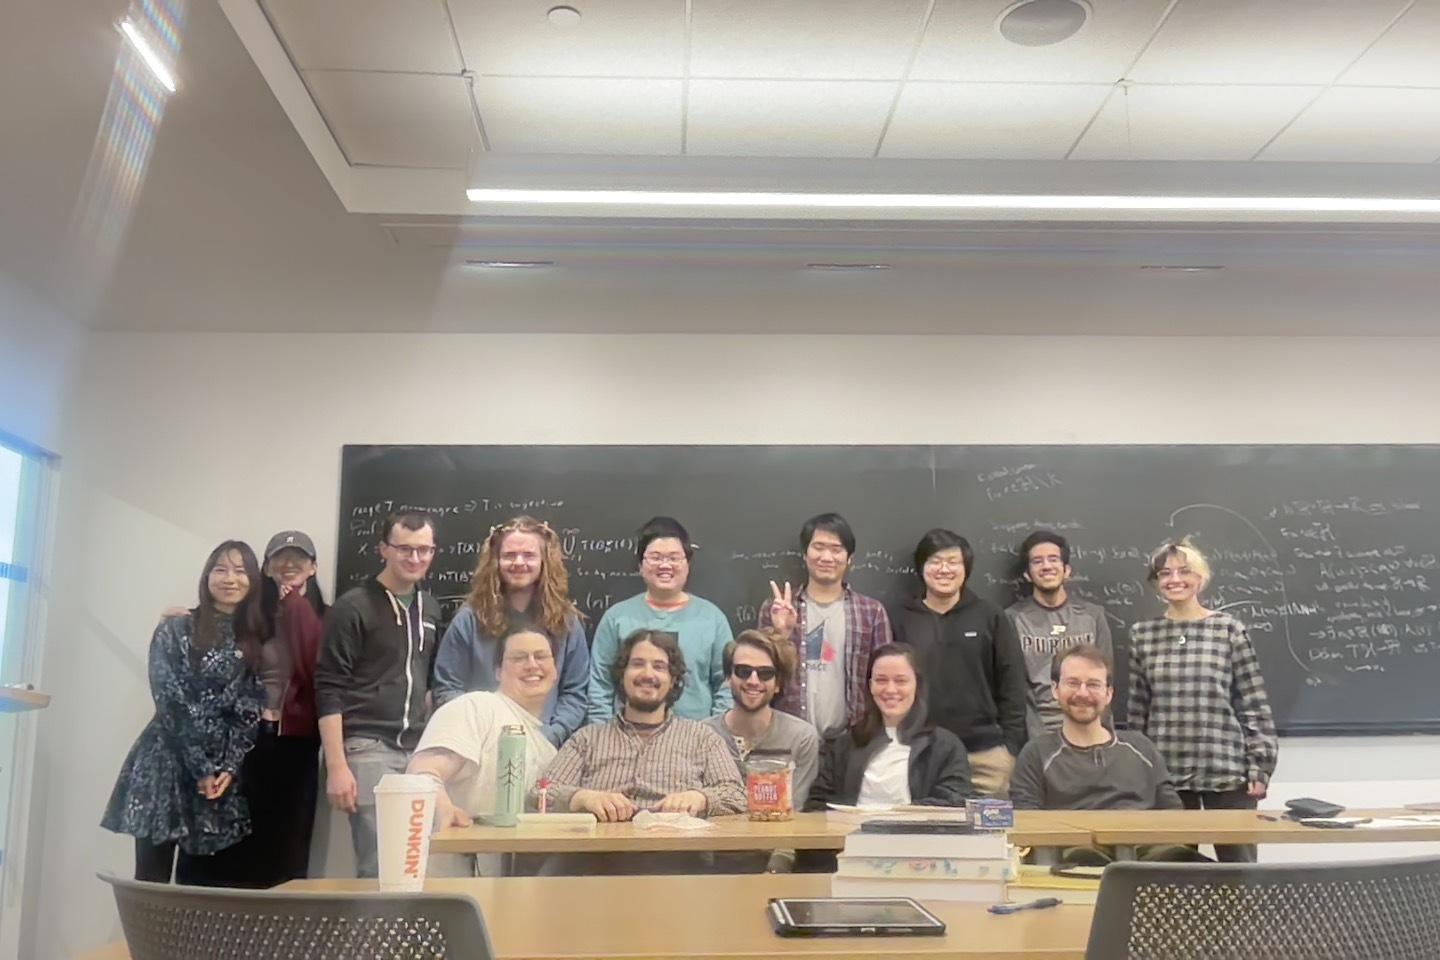
\includegraphics[width=150mm]{FuNtional exam group.jpg}
    My main collobarators were Scott, Eric, Josh, Ishaan, Vievie, Satchel, and Danny, however problems were likely mentioned and discussed to some degree with essentially all individuals in the picture.
\end{thebibliography}

\end{document}